\documentclass[12pt,a4paper,twoside]{article}

\usepackage[colorlinks=true,urlcolor=blue,linkcolor=blue]{hyperref} 
\usepackage{fancyhdr}
\usepackage{lastpage}
\usepackage{a4wide} 
\usepackage{amsmath}
\usepackage{amssymb} 
\usepackage{graphicx}
\usepackage{color}
\usepackage{fancybox}
\usepackage{moreverb}
\usepackage[default]{lato}
\usepackage[T1]{fontenc}
% \usepackage{hangcaption}
\usepackage{placeins} % For FloatBarrier
\usepackage[utf8]{inputenc}
\usepackage[english]{babel} % To have \tableofcontents translated by Table des matières
\usepackage{listings}

\newcommand{\myparagraph}[1]{\paragraph{#1}\mbox{}\\}

%\fbox{}
%\shadowbox{}
%\doublebox{}
%\ovalbox{}
%\Ovalbox{}
%\shabox{}

\title{Specifications}
\author{Grosjean Nicolas}
\date{\today}

\pagestyle{headings}

\begin{document}
\lstset{ numbers=left, tabsize=3, frame=single, numberstyle=\ttfamily, basicstyle=\footnotesize} 
\thispagestyle{empty}

\begin{center}
\vspace{3cm}
{\LARGE Specifications}\\
\vspace{1cm}
Work in progress\\
\vspace{2cm}
\shadowbox{
\begin{minipage}{1\textwidth}
\begin{center}
{\Huge Timeline}\\
\end{center}
\end{minipage}
}\\
\vspace{1cm}
\FloatBarrier
\begin{figure}[ht]
\centering 
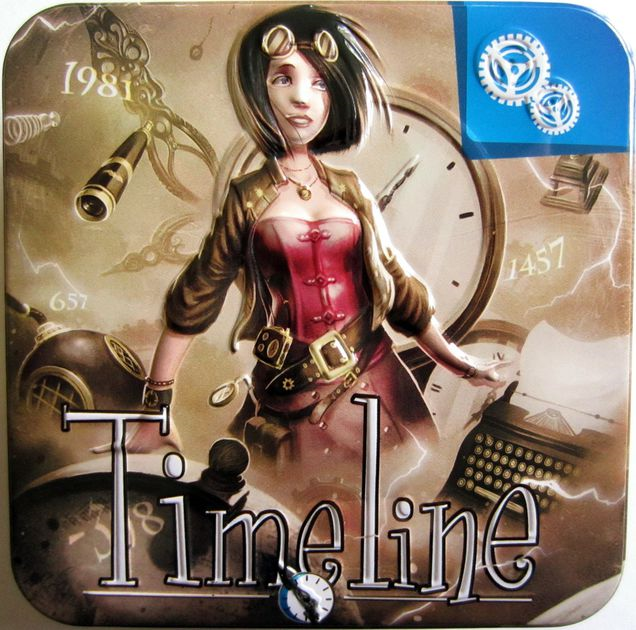
\includegraphics[scale=0.5]{Images/Timeline.png}
\end{figure}
\FloatBarrier
\vspace{1cm}
\begin{tabular}{p{10cm}p{10cm}}
{\bf Open Source Project}                                            &{\bf Author}\\
{\footnotesize C++}       & ~~~Nicolas Grosjean (a.k.a Mouchi)\\
{\footnotesize }                                        & {\bf Contributor}\\
{\footnotesize }                          & ~~~Maxime Deroin
\end{tabular}
\end{center}


\newpage
\tableofcontents
\newpage

\section{Abstract}

\subsection{The project}
The project aims to learn things in C++ and tools by practise.\\
It is also the occasion to have an implementation of the good board-game TimeLine and to go further.

\subsection{Project management}
\textbf{The project management is on the GitHub website} and so is opened to the community.\\
The project will be structured on \textbf{iteration} also called \textbf{milestone} on GitHub. Each milestone correspond to an amount of features which represent an important step in the development.\\
The objective is to do milestones in the order but we can implement some features of the next milestone to advance.\\
When a milestone is over, if the game is stable, we will proceed to a release.

\vspace{5mm}

For the detail of an iteration, the \textbf{features}, we will use the \textbf{issues} on GitHub .\\
We will use a Kanban table to classify the issues according their state (TODO, In Progress, To Validate, Done).\\
So when an issue is created, its state is TODO.\\
If an issue is on the TODO state and not assigned, we can assign it to oneself to avoid someone works also on it.\\
Then when somebody is working on the issue, its state is In Progress.\\
When the development is done, the issue becomes To Validate state. Someone else should validate the development. It is the occasion for the commiter and the reviewer to learn from each other.\\
Finally when the issue is validated it is done. It can be removed from the table when its content is in a release.

\vspace{5mm}

We will use tools to improve the code quality : unit test framework, code analyser ...

\vspace{5mm}

Like the main objective is to learn, all the features and so the iterations will not be done.

\newpage

\section{Iterations}

\subsection{Minimal interactive game}

The minimal interactive game is a \textbf{solo} game where the user try to put 5 cards of events in the good chronological order whereas a 6th card is already placed in the table.\\
The 6th card is in the \textbf{middle} on the game with the \textbf{year} of the event visible.\\
The 5 cards of the user are at the \textbf{bottom}, the years of the events are not visible. The user can \textbf{drag and drop} one card to the middle to put it at the left, at the right or between the other cards of in the middle. By doing that, the year of the card will be visible. If the card is correctly set according chronological order, it stays. Otherwise it is removed.\\
When there is no more cards in the bottom, the game is over.

The cards and the years are get from images and their file name.
The image should be defined in order to they all have it.

\subsection{Ideas for the next iterations}
\begin{itemize}
\item Score the card correctly placed
\item Save the scores to compute some statistics (max, mean, number of games)
\item Take randomly the cards in a directory
\item Choose the directory in which take the cards
\item Choose the number of cards in the middle and at bottom in the beginning
\item Multi-player game
\item New game mod : see \href{https://www.trictrac.net/actus/timeline-challenge-le-comment-ca-marche}{Timeline Challenge}
\end{itemize}

\end{document}